\documentclass[brudnopis]{xmgr}

\definecolor{sa}{cmyk}{0,1,0.13,0}
\definecolor{sb}{cmyk}{0.99,0,0.52,0}
\definecolor{sc}{cmyk}{0,0.75,1,0.24}
\definecolor{wa}{cmyk}{0,1,0.13,0}
\definecolor{wb}{cmyk}{0.99,0,0.52,0}
\definecolor{wc}{cmyk}{0,0.75,1,0.24}
\definecolor{wd}{cmyk}{0.98,0.13,0,0.43}
\definecolor{stressp}{cmyk}{0,1,0.13,0}
\definecolor{topicp}{cmyk}{0.98,0.13,0,0.43}

%\defaultfontfeatures{Scale=MatchLowercase}
%\setmainfont[Numbers=OldStyle,Ligatures=TeX]{Minion Pro}
%\setsansfont[Numbers=OldStyle,Ligatures=TeX]{Myriad Pro}
% for fontspec version < 2.0
\setmainfont[Numbers=OldStyle,Mapping=tex-text]{Minion Pro}
\setsansfont[Numbers=OldStyle,Mapping=tex-text]{Myriad Pro}
%\setmonofont[Scale=0.75]{Monaco}

% Opcjonalnie identyfikator dokumentu
% drukowany tylko z~włączoną opcją 'brudnopis':
\wersja   {wersja wstępna [\ymdtoday]}

\author   {Mateusz Kwiatkowski}
\nralbumu {194\,925}
\email    {emflover@gmail.com}

\kierunek{\textbf{INFORMATYKA}}

\title    {Walidacja w~elektronicznym systemie zarządzania osiągnięciami studenta}
\date     {2014}
\miejsce  {Gdańsk}

\opiekun  {dr Włodzimierz Bzyl}

% dodatkowe polecenia

\begin{document}

\begin{abstract}

\begin{description}
\item[sa] \textcolor{sa}{powinno zawierać omówienie głównych
tez pracy magisterskiej, celów jakie autor sobie postawił}
\item[sb] \textcolor{sb}{powinno zawierać informację czy udało
  się je zrealizować}
\item[sc] \textcolor{sc}{należy także napisać jakimi metodami,
  technologiami się posłużono i~jakie to przyniosło efekty}
\end{description}

\indent \indent \textcolor{sa}{Pracę poświęcono zagadnieniu walidacji, kwestii ważnej i~integralnie związanej z~odpowiednim funkcjonowaniem sieci.
W szczególności zwrócono uwagę na aspekt prawidłowego zarządzania jej jakością, co obligatoryjnie wiąże się z~problemem
odpowiedniego zabezpieczenia i~odpowiedzialnego korzystania z~niej.}
\\
\indent \textcolor{sa}{Praca prezentuje sposób tworzenia oraz funkcjonowanie pakietu walidującego do frameworka \textit{Meteor}. Pakiet ten
ma uniemożliwić użytkownikowi wprowadzenie błędnych danych do systemu, dzięki czemu podniesiony zostanie poziom zaufania
do korzystania z~niego. Jednocześnie, aby przybliżyć i~zademonstrować jego działanie, utworzono na potrzeby pracy, aplikację elektroniczny indeks.
Wybór dokumentu nie był przypadkowy. Świadczy o~tym jego wysoka ranga wśród uczelnianej dokumentacji urzędowej. Inny, równie istotny powód
wyboru stanowi fakt, iż korzystanie z~sieci komputerowej w~systemie edukacyjnym stało sie powszechne. Uczelnie wyższe wykorzystują sieć, by
między innymi ułatwić kontakty na linii: wykładowca - student - administracja uczelni.  Temu ma służyć wprowadzenie w~ostatnich latach przez
większość uczelni wyższych w~Polsce, w~tym Uniwersytet Gdański, elektronicznego systemu zarządzania osiągnieciami studentów
tzw. elektronicznego indeksu.}
\\
\indent \textcolor{sc}{W pracy, walidacji zostaną poddane operacje, które można wykonać w~aplikacji elektroniczny indeks. Do stworzenia jej użyto frameworku \textit{Meteor}, a~dane wprowadzone do systemu, w~celu ich przechowywania umieszczono w~bazie danych - \textit{MongoDB}.}
\\
\indent \textcolor{sb}{Założono, że skutkiem tego informatycznego sofizmatu będzie uproszczenie, a~nawet intuicyjność obsługi oprogramowania. Cele założone przez autora pracy zostały zrealizowane, czego dowodem jest udostepnienie do pobrania pakietu walidacji systemu.}

\end{abstract}
%\keywords{SGML,
% dokumenty strukturalne}

% tytuł i~spis treści
\maketitle
%
% wstęp
\introduction

\begin{description}
\item[wa] \textcolor{wa}{jak nazwa wskazuje, ma wprowadzać
  w~obszar problemowy pracy}
\item[wb] \textcolor{wb}{powinno przedstawiać ogólne
  uwarunkowania problemu oraz opisać go w kontekście}
\item[wc] \textcolor{wc}{powinno zawierać powód dlaczego
  poruszyło się taki temat}
\item[wd] \textcolor{wd}{należy odnieść się do dorobku innych}
\end{description}

\indent \indent \textcolor{wa}{Najcenniejszym walorem komputera i~Internetu są przechowywane w~nich dane - zarówno
ich ilość, jak i~jakość. Ze względu na to, z~dnia na dzień, rośnie liczba
użytkowników sieci. Jednocześnie zwiększa się liczebność i~różnorodność usług
sieciowych.}
\\
\indent \textcolor{wa}{Komputer i~Internet zmienił, wciąż zmienia naszą codzienność. To prawda oczywista.
Usługi internetowe nie są już domeną urzędów, firm czy handlu. Chcemy za ich pomocą
robić zakupy, obsługiwać konto w~banku, a~także załatwiać wszelkie formalności w
urzędach. Jest to po prostu wymóg rozwoju cywilizacji, techniki oraz oszczędności
czasu.}
\\
\indent \textcolor{wa}{Coraz częściej systemy informatyczne wykorzystywane są w~edukacji społeczeństwa.
Jeszcze do niedawna na wszystkich uczelniach wyższych stosowano klasyczne indeksy
papierowe, aby zarchiwizować osiągnięcia studentów podczas całego cyklu kształcenia.
Jednak w~wyniku rozwoju technologii internetowych coraz częściej rezygnuje się
z klasycznych rozwiązań, zastępując je ich elektronicznymi odpowiednikami.}
\\
\indent \textcolor{wb}{Dziś wiele szkół i~uczelni wprowadziło do obszaru swego funkcjonowania nowoczesny
system ewidencji osiągnięć ucznia czy studenta. W~szkołach podstwowych, gimnazjach,
liceach, technikach czy zasadniczych szkołąch zawodowych jest nim tzw. dziennik
elektroniczny. W~uczelniach wyższych  nazwano go elektronicznym indeksem. Zjawisko
to stanowi nie lada wyzwanie, ponieważ wiąże się z~problemem niezawodnego świadczenia
usług w~sieci komputerowej. Odbiorca, w~tym przypadku uczeń lub student, musi mieć
pewność, że dane są stałe, prawdziwe, odpowiednio zabezpieczone przed ich utratą
czy nieuprawnionym dostepem. Należy nadmienić, że taki poziom zaufania i~poczucia
bezpieczeństwa funkcjonowania systemu, powinna mieć również druga strona - nadawca,
ten który wprowadza owe dane. Jest to tym bardziej ważną kwestią, gdyż coraz częściej
mamy do czynienia ze zdarzeniami, wskazującymi na nieprawidłowe stosowanie sieci
komputerowej lub jej nadużycie.}
\\
\indent \textcolor{wa}{Rozwiązaniem, które zapewniłoby wzrost poziomu zaufania do korzystania
\\
z sieci,
w tym również z~elektronicznego systemu zarządzania osiagnieciami ucznia lub studenta
jest, według autora niniejszej pracy, odpowiednie i~odpowiedzialne zarządzanie jej
jakością, czemu służy walidacja systemu.}
\\
\indent \textcolor{wa}{Zjawisko to jest szeroko stosowane w~technice i~informatyce. Internetowy Słownik
Języka Polskiego wyjaśnia hasło ,,walidacja'' w~następujacy sposób: ,,walidacja
(technika) - badanie odpowiedności, trafnośc lub dokładności czegoś''.\cite{ValidationSJP}}
\\
\indent \textcolor{wa}{Sam termin - ,,walidacja'' pochodzi od angielskiego słowa ,,validate'' i~oznacza -
w kontekście informatycznym - sprawdzanie poprawności i~zgodności z~zadanymi
kryteriami. Jest on stosowany w~odniesieniu do danych pochodzących od użytkownika,
jak również w~stosunku do zmiennych, obiektów, typów i~klas w~różnych językach
programowania.\cite{ValidationTermin}}
\\
\indent \textcolor{wa}{Walidacja jest działaniem, mającym na celu potwierdzenie w~sposób udokumentowany
i zgodny z~założeniami, że procedury, procesy, urządzenia, materiały, czynności
i systemy, rzeczywiście prowadzą do zaplanowanych wyników. Znana jest także jako
kontrola jakości oprogramowania.\cite{Validation2}}
\\
\indent \textcolor{wa}{Wprowadzając dane do systemu, użytkownik może - świadomie lub nie - popełnić
pomyłkę. Jeżeli dane odebrane przez użytkownika poddamy przetworzeniu bez weryfikacji,
wówczas, w~zależności od odporności aplikacji, możemy mieć do czynienia z~różnymi
rodzajami błędów, od drukowania w~przeglądarce klienta komunikatów diagnostycznych,
poprzez utratę spójności bazy danych, aż po ujawnienie niepowołanym użytkownikom
informacji poufnych. Z~tego powodu nie wolno ignorować wagi problemu.}
\\
\indent \textcolor{wc}{Aplikacje pozbawione walidacji pozwalają użytkownikowi na wprowadzenie irracjonalnych
danych do systemu. Przykładem takiej aplikacji jest wspomiany przez autora pracy,
elektroniczny indeks. Operacje, takie jak: wystawianie studentowi ocen z~ćwiczeń
czy też oceny z~egzaminu kończącej edukację z~danego przedmiotu, powinny być
odpowiednio walidowane. Dzięki temu nie dojdzie do niepożądanych zjawisk typu:
\begin{itemize}
\item student nie uzyskał pozytywnej oceny z~ćwiczeń, a~otrzymuje ocenę z~egzaminu
kończącego przedmiot,
\item student otrzymuje ocenę spoza skali oceniania systemu danej uczelni,
\item student uzyskuje ocenę od osoby nieuprawnionej do jej wystawienia.
\end{itemize}}

\textcolor{wc}{Dlatego też, autor pracy chce zwrócić uwagę na rodzący się problem, związany
z wprowadzeniem przez uczelnie elektronicznego indeksu oraz jego odpowiednim
funkcjonowaniem. Zaproponowanie zastosowania walidacji w~elektronicznym systemie
wystawiania ocen usprawni działanie oraz udoskonali jego funkcjonalność.
Korzystając z~aplikacji, w~której zaimplementowana jest walidacja możemy mieć pewność,
że nie dojdzie do sytuacji, by użytkownik wprowadził błędne dane do systemu.
Należy również zwrócić uwagę na ekonomiczny aspekt walidacji. Mianowicie oszczędność
czasu użytkownika czy zwiększenie efektywności jego pracy.}
\\
\indent \textcolor{wc}{W celu ukazania i~udowodnienia przydatności walidacji podczas korzystania
z elektronicznego systemu zarządzania osiągnięciami studenta, pokazano w~pracy
działanie tego zjawiska w~aplikacji stworzonej w~frameworku \textit{Meteor} oraz
zaprezentowano ułożony pakiet oraz wyjaśniono, jak udostępnić go w~prosty, jasny i~zrozumiały sposób.}
\\
\indent \textcolor{wd}{Tworzenie pakietu walidującego oraz aplikacji - elektroniczny indeks, która korzysta
ze stworzonego w~ramach pracy pakietu, oparto na doświadczeniu innych badaczy,
zajmujących się oprogramowaniami komputerowymi, takich jak: Kelly Copley, Tom
Coleman czy Sacha Greif.} \textcolor{wa}{W pracy umieszczono ponadto uzasadnienie, dlaczego wybrane
technologie, takie jak - \textit{Meteor} oraz \textit{MongoDB}, to najbardziej trafny wybór do generowania
pakietu walidacyjnego elektronicznego zarządzania osiągnięciami studenta.}
\\
\indent \textcolor{wa}{Autor niniejszej pracy miał kontakt z~wieloma systemami zarządzania osiągnieciami
studentów, ale w~każdym można było doprowadzać do anomalii. Zajęcie się rozwiązaniem
tego problemu jest, z~punktu widzenia informatyka interesujące. Efektem pracy może być
nie tylko usprawnienie działania systemu, ale również poczucie, że praca z~nim jest
prosta, przyjemna i~wręcz intuicyjna.}





\chapter{Walidacja oprogramowania}

\begin{description}
\item[stressp] \textcolor{sa}{Najbardziej istotna informacja}
\item[topicp] \textcolor{sb}{Początek nowego zdania odnoszący sie do istotnej informacji poprzedniego zdania}
\end{description}

\indent \indent \indent \textcolor{sb}{W testowaniu oprogramowania ważne są pojęcia – weryfikacja i~walidacja.} \textcolor{sa}{Pojęcie walidacji wyjaśniono we wprowadzeniu oraz rudymencie podrozdziału pierwszego.} \textcolor{sb}{Należy wyjaśnić również pojęcie \textit{weryfikacji}}

\textcolor{sa}{\textit{Internetowy Słownik Języka Polskiego} podaje następujące znaczenia tego słowa: \textit{weryfikacja} z~łac. \textit{verifico} - ,,wycenić wartość, ustalić; 1. Sprawdzenie zgodności czegoś z~prawdą; sprawdzenie autentyczności czegoś; weryfikacja hipotezy, teorii, faktów. 2. Sprawdzanie i~ocena czyichś kwalifikacji - np. pracownika''.} \textcolor{sb}{Różnica w~znaczeniu tych pojęć jest istotna.} \textcolor{sa}{Aby ją wskazać należy zwrócić uwagę na celowość tych dwóch określeń.} \textcolor{sb}{Specyfika działania weryfikacji to zastosowanie pytania:} \textcolor{sa}{\textit{,,Czy produkt tworzony jest prawidłowo?''}.} \textcolor{sb}{Z kolei dla procesu walidacji typowym pytaniem będzie:} \textcolor{sa}{\textit{,,Czy tworzony produkt jest prawidłowy?''}.} \textcolor{sb}{\textit{Prawidłowy} – to znaczy} \textcolor{sa}{zgodny z~wytycznymi programowania, przy zastosowaniu odpowiednich metod, języka programowania i~algorytmów. }

\textcolor{sb}{Pojęcia weryfikacji i~walidacji są znaczeniowo na tyle bliskie, że mogą przysporzyć trudności.} \textcolor{sa}{Zarówno weryfikacja jak i~walidacja produktu są czynnościami, które służą sprawdzeniu,} \textcolor{sb}{czy wytworzony produkt jest taki, jaki sobie życzyliśmy my, bądź inny interesariusz.} \textcolor{sa}{\textit{Produkt} możemy rozumieć jako: }

\begin{itemize}
  \item[-] \textcolor{sa}{dany moduł systemu,}
  \item[-] \textcolor{sa}{blok kodu,}
  \item[-] \textcolor{sa}{cały system,}
  \item[-] \textcolor{sa}{istotny dokument, na bazie którego moduł lub system będzie zbudowany.}
\end{itemize}

\textcolor{sb}{Warto zapamiętać, że obie te czynności zachodzą w~wielu różnych momentach i~mogą pojawić się w~wielu fazach procesu tworzenia systemu.} \textcolor{sa}{Błędnym będzie zatem rozumienie, np. walidacji, jako jakiegoś etapu wieńczącego budowę systemu.}

\begin{figure}[th!]
\centering
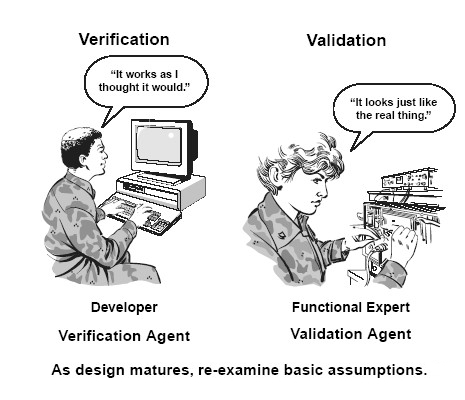
\includegraphics[width=.7\hsize]{images/Verification_Validation_Accreditation}
\caption{Różnice między weryfikacją, walidacją\label{RYS.1}}
\source{http://commons.wikimedia.org/wiki/}
\end{figure}

 \textcolor{sb}{Różnice między weryfikacją i~walidacją dotyczą przede wszystkim tego, z~jakiej perspektywy dokonujemy sprawdzenia} \textcolor{sa}{czy jest to perspektywa technologiczna i~typowa dla zespołów budujących system, czy raczej z~perspektywy użytkownika końcowego, który nie ma obowiązku rozumieć technicznej strony systemu, z~którego będzie korzystał.}
\\
\indent \textcolor{sb}{Najprościej jest zapamiętać, że weryfikujemy to,} \textcolor{sa}{co da się wyliczyć, wykazać logicznie i~nie ma jak zanegować tego, co już zweryfikowane.} \textcolor{sb}{Przy dobrze spisanych wymaganiach} \textcolor{sa}{weryfikacji dokonać może każdy człowiek rozumiejący tekst specyfikacji i~wiedzący, jak wykonać test. }
\textcolor{sb}{Natomiast walidacja zawsze jest po stronie odbiorcy i} \textcolor{sa}{to zaspokojenie jego potrzeb jest ostatecznym kryterium sukcesu.} \textcolor{sb}{Odcinając się od możliwości konsultowania z~klientem spraw dotyczących choćby wygody użytkowania produktu,} \textcolor{sa}{wytwórcy ryzykują niepowodzenie walidacji.}
\\
\indent \textcolor{sb}{Weryfikacja produktu procesu} \textcolor{sa}{polega na dostarczeniu dowodów, że dany produkt spełnia z~d~e~f~i~n~i~o~w~a~n~e wymagania.} \textcolor{sb}{Można spotkać się też z~objaśnieniami tego terminu mówiącymi, że} \textcolor{sa}{jest to sprawdzanie „czy aplikacja jest prawidłowo zbudowana”, czy produkty danego etapu produkcji spełniają wymogi założone na początku całego procesu.}
\textcolor{sb}{Kluczowym słowem jest wyraz -  \textit{zdefiniowane}.} \textcolor{sa}{Weryfikacja domaga się odniesienia do przesłanek, które spisano w~taki sposób, by można je było sprawdzić w~sposób jednoznaczny.} \textcolor{sb}{Weryfikacja polega na stwierdzeniu, że dany punkt np. specyfikacji technicznej jest informacją,} \textcolor{sa}{która w~sposób prawdziwy opisuje dany produkt poddany testowi.} \textcolor{sb}{W praktyce powinniśmy zatem unifikować weryfikację z~procesem, który zakończy się „zero-jedynkowym” rozstrzygnięciem,} \textcolor{sa}{decydującym o~tym, że dany produkt wygląda, bądź zachowuje się, bądź jest taki, jak ustalono dla niego w~specyfikacji wszystkich przesłanek.} \textcolor{sb}{Jeśli na przykład jakąś funkcjonalność można:}
\begin{itemize}
  \item[-] \textcolor{sa}{sprawdzić poprzez odczytanie wyniku liczbowego, którego ona dostarcza; }
  \item[-] \textcolor{sa}{zbadać czy odpowiedź systemu nastąpi w~konkretnie ustalonym czasie;}
  \item[-] \textcolor{sa}{sprawdzić czy następuje przesłanie odpowiedniego pliku między serwerem a~klientem,
wtedy możemy oczekiwać, że proces sprawdzania tego produktu jest weryfikacją.}
\end{itemize}


\begin{figure}[th!]
\centering
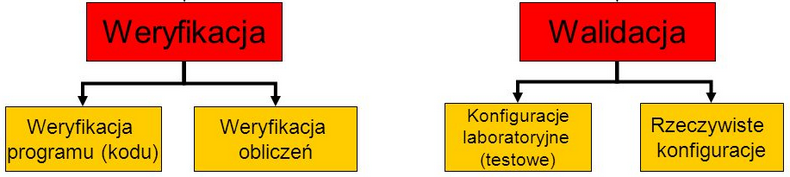
\includegraphics[width=.7\hsize]{images/weryfikacja_walidacja}
\caption{Weryfikacja i~walidacja\label{RYS.2}}
\source{http://slideplayer.pl/slide/427709/ slajd 4}
\end{figure}

\indent \textcolor{sb}{Walidacja produktu polega na} \textcolor{sa}{sprawdzeniu poprawności i~dostarczeniu dowodów,  że proces wytwarzania go, spełnia potrzeby i~wymagania użytkownika. Tłumaczy się ją również, jako „sprawdzenie czy aplikacja jest poprawna” / w~starszych wersjach słowników testerskich /}\cite{ALTKOM}
\\
\indent \textcolor{sb}{Najistotniejsze do zrozumienia walidacji jest to,} \textcolor{sa}{że to, co było jasno zdefiniowanym kryterium zaliczenia testu, jest tutaj zamienione na potrzeby i~wymagania użytkownika.} \textcolor{sb}{O ile zweryfikować można różne rzeczy bez wczuwania się w~rolę użytkownika końcowego / bo wystarczy się oprzeć choćby na wyliczeniach i~sprawdzaniu, czy wyniki są zgodne z~założeniami ze specyfikacji /,} \textcolor{sa}{to walidacja służy właśnie do sprawdzenia wszystkich tych funkcjonalności, które użytkownik będzie oceniał pod kątem swoich osobistych upodobań, często subiektywnie, nieraz w~oparciu o~rozmaite nawyki.}
\textcolor{sb}{Sukces walidacji opiera się niejednokrotnie na sprawach,} \textcolor{sa}{które ciężko jest przewidzieć podczas pisania specyfikacji funkcjonalnej.} \textcolor{sb}{Odbiorca systemu nieraz nie uświadamia sobie swoich własnych aberracji} \textcolor{sa}{i~może stwierdzić ich brak dopiero wtedy, gdy przystępuje do finałowego testu akceptacyjnego.} \textcolor{sb}{Często wtedy słyszanym argumentem z~ust niezadowolonego odbiorcy jest to,} \textcolor{sa}{że coś było „tak oczywiste, że nie trzeba tego było spisywać w~specyfikacji”.}
\textcolor{sb}{O ile kluczem do udanej weryfikacji produktu jest klarowne zdefiniowanie kryteriów zaliczenia testu,} \textcolor{sa}{o tyle kluczem do udanej walidacji jest pogłębiona i~sprawna komunikacja z~odbiorcą, zadawanie celnych pytań pomagających w~zrozumieniu autentycznych potrzeb klienta, przeprowadzanie wraz z~klientem symulacji zastosowań systemu na wszelkiego rodzaju makietach.} \textcolor{sb}{Kolejną bardzo istotną sprawą jest umiejętne korzystanie z~badań aktualnych rozwiązań i~tendencji w~produktach dostępnych na rynku,} \textcolor{sa}{co wiąże się z~przeglądaniem odpowiednich stron internetowych, sięganiem po prace znawców tematu i~autorytetów, ciągłym dokształcaniem.}
\\
\indent \textcolor{sb}{Walidację warto zapamiętać jako ogół tych czynności, które zwiększają szansę na zadowolenie odbiorcy tworzonego produktu i~które będą brały pod uwagę konsultacje z~tym odbiorcą,} \textcolor{sa}{wspólne wypracowywanie rozwiązania i~przewidywanie jego preferencji.}\cite{ALTKOM}

\section{Specjalistyczny rudyment do walidacji}

\indent \indent \indent \textcolor{sb}{Walidacja jest to proces wyznaczania kompatybilności stopnia użytkowania systemu,} \textcolor{sa}{w którym dany model staje się wiernym odzwierciedleniem rzeczywistego systemu.} \textcolor{sb}{Chodzi o~skuteczną zgodność wprowadzonych danych z~ich oryginałem.} \textcolor{sa}{Proces ten ma na celu zilustrowanie czy symulacja dostarcza użytkownikowi wiarygodnych danych wyjściowych, zgodnych z~danymi wejściowymi użytkownika. Dokonuje więc, weryfikacji zgodności wizji projektanta z~realnym światem. Pełni rolę autocenzury konkretnego systemu, by każdy wirtualny użytkownik, miał pewność, że dane wprowadzone do systemu są stałe i~spełniają przydzieloną im rolę.}
\\
\indent \textcolor{sb}{Każdy system informatyczny wymaga osiągnięcia odpowiedniego stopnia adekwatności, bezbłędności, stabilności oraz wyeliminowania błędów działania w~modelu}. \textcolor{sa}{Przez model, który przeszedł walidację, rozumieć należy ten, który został poddany serii operacji,} \textcolor{sa}{mających na celu doprecyzowanie go do optymalnego poziomu, przez co, zgodnie z~jego przeznaczeniem, będzie mógł sprostać postawionym przed nim zadaniom. Taki poziom wiarygodności modelu uzyskamy dzięki procesowi walidacji.}

\textcolor{sb}{Systemy zautomatyzowane i~skomputeryzowane stosowane szczególnie w~przemyśle wysokich technologii, muszą być poddawane okresowym kontrolom,} \textcolor{sa}{potwierdzającym ich jakość w~celu wykrycia ewentualnych, potencjalnych zagrożeń, wynikających z~bezpośredniego lub pośredniego wpływu na produkt końcowy. Walidacja zatem ma udokumentować, w~jaki sposób należy zmienić i~udoskonalić proces, aby zminimalizować ewentualne skutki jego nieprawidłowego działania.}

\textcolor{sb}{Jeżeli istnieje możliwość, walidacja systemu powinna być poprzedzona rozmową z~jego użytkownikiem.} \textcolor{sa}{Ma ona spełnić rolę sondy i~zebrania cennych informacji, by program walidacyjny stał się optymalny.} \textcolor{sb}{Mając przez długi czas styczność z~systemem rzeczywistym, ekspert często potrafi odpowiedzieć na pytania dotyczące całości systemu lub wskazać rażące błędy,} \textcolor{sa}{których podstawą jest niezrozumienie rzeczywistego systemu, co staje się przyczyną generowania przez symulację złych wyników.} \cite{Validation}

\indent \textcolor{sb}{Innym zagadnieniem mającym związek z~procesem walidacji jest problem czasu tworzenia go oraz związanych z~tym kosztów.} \textcolor{sa}{Walidacja procesów,systemów czy urządzeń jest czasochłonna. Tworzenie dokumentacji, procedur, wykonywanie testów i~działań naprawczych na ogół przeciąga się w~czasie.} \textcolor{sb}{Dobrze zarządzana walidacja, obciąża budżet projektu w~skali 4 - 7 \% kosztów.} \textcolor{sa}{Nieprawidłowo prowadzona podnosi ją do 20 – 30\% kosztów całkowitych.} \textcolor{sb}{Poniesienie niskich nakładów może przynieść wymierne zyski ekonomiczne już w~krótkiej perspektywie.} \textcolor{sa}{Według danych zgromadzonych przez osoby zajmujące się walidacją dla nowych urządzeń i~systemów produkcyjnych, wydajność początkowa urządzenia, które były przedmiotem pełnego cyklu walidacji, może być 2 – 3 razy wyższa, niż tych uruchomionych bez jej przeprowadzania.} \textcolor{sb}{Mechanizmy i~systemy poddane walidacji osiągają pełną zdolność produkcyjną a~ich kultura obsługi i~serwisu jest wysoka,} \textcolor{sa}{ponieważ w~czasie testów walidacyjnych pracownicy zdobywają praktyczną wiedzę od dostawcy czy użytkownika.} \textcolor{sb}{Właściwe opracowanie \textit{specyfikacji wymagań użytkownika}
\\
/ w~skrócie URS / \footnote{ang. User Requirements Specification - URS}, prowadzenie kwalifikacji projektu, nadzorowanie i~współpraca z~dostawcą} \textcolor{sa}{od początku wiąże się z~nakładami.} \textcolor{sb}{Jednak poniesione koszty są niewspółmierne niższe od kosztów poprawy pracy czy usuwania usterek w~gotowym urządzeniu, czy utworzonym systemie.} \textcolor{sa}{Dlatego ważna jest współpraca z~dostawcą / użytkownikiem  od samego początku inwestycji.} \textcolor{sb}{Wspólne rozwiązywanie problemów, tworzenie scenariuszy testowych,} \textcolor{sa}{pozwala na obustronną wymianę wiedzy
\\
i znaczne ograniczenie kosztów w~późniejszej eksploatacji systemu i~urządzenia.}\cite{ekonomia}

\section{Kategorie walidacji}

\textcolor{sb}{Kryterium funkcjonalności wyróżnia następujący podział walidacji:}

\begin{enumerate}
  \item \textbf{\textit{Walidacja prospektywna}} – \textcolor{sa}{zadaniem takiej walidacji jest, aby przed wprowadzeniem nowych produktów na rynek upewnić się, że funkcjonują prawidłowo i~spełniają standardy bezpieczeństwa.}
  \item \textbf{\textit{Walidacja retrospektywna}} – \textcolor{sa}{ten proces wyasygnowano dla produktów, które są już w~użyciu oraz dystrybucji czy produkcji. Walidację tą przeprowadza się na podstawie wcześniej określonych oczekiwań specyfikacji produktu oraz danych historycznych. Jeśli jakiekolwiek dane krytyczne są niepełne, to nie mogą być one przetworzone lub mogą być przetworzone częściowo.} \textcolor{sb}{Zadania są uważane za konieczne, gdy:}
\begin{itemize}
\item \textcolor{sa}{walidacja prospektywna jest niewystarczająca lub błędna,}
\item \textcolor{sa}{zmiana przepisów prawnych lub norm wpływa na zgodnośc produktów wypuszczonych na rynek,}
\item \textcolor{sa}{przywrócenie produktu do użytkowania.}
\end{itemize}
  \item \textbf{\textit{Rewalidacja}} – \textcolor{sa}{przeprowadza się dla produktu, który został odrzucony, naprawiony, zintegrowany, przeniesiony lub po upływie określonego czasu.}\cite{Categories}
\end{enumerate}

\section{Etapy walidacji}
\indent \indent \indent \textcolor{sb}{Zakres walidacji powinien uwzględniać wiele czynników systemu,} \textcolor{sa}{w tym jego zamierzone zastosowanie i~rodzaj walidacji oraz czy mają być dołączane nowe elementy systemu.} \textcolor{sb}{Walidacja powinna być uznawana za część całego cyklu użytkowania systemu komputerowego.} \textcolor{sa}{Cykl ten obejmuje planowanie, specyfikację, programowanie, badanie, odbiór techniczny, dokumentację, działanie, monitorowanie i~modyfikowanie.}

\begin{figure}[th!]
\centering
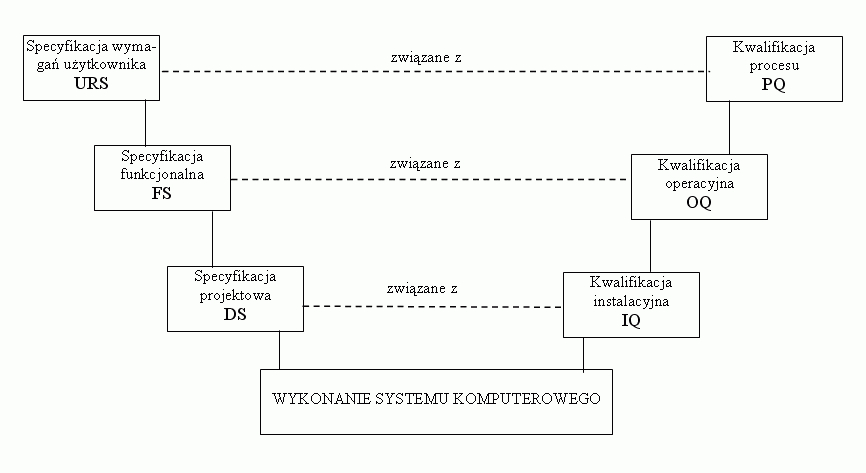
\includegraphics[width=.7\hsize]{images/cykl}
\caption{Cykl życia systemu\label{RYS.3}}
\source{http://www.label.pl}
\end{figure}

\textcolor{sb}{Projektowanie systemu skomputeryzowanego można podzielić na kilka etapów:}

\begin{enumerate}
  \item \textbf{\textit{Specyfikowanie}} – \textcolor{sa}{URS oraz specyfikacja funkcjonalna\footnote{ang. Functional Specification - FS}. W~planie walidacji tego etapu projektowania powinno się uwzględnić audyt dostawcy oraz przegląd specyfikacji.}
  \item \textbf{\textit{Projektowanie}} – \textcolor{sa}{projekt hardwaru\footnote{ang. Hardware Design System - HDS}, softwaru\footnote{ang. Software Design System - SDS}, projekt mechaniczny i~elektryczny oraz projekt sieci informatycznej. Walidacją objęty jest przegląd poszczególnych projektów – kwalifikacja projektu\footnote{ang. Design Qualification - DQ}.}
  \item \textbf{\textit{Wykonanie}} – \textcolor{sa}{utworzenie hardwaru, połączeń elektrycznych modułów systemu, oprogramowanie modułów, montaż całego urządzenia, wykonanie sieci informatycznej. Walidacja obejmuje przeglądy wykonania poszczególnych czynności oraz przegląd kodów źródłowych oprogramowania.}
\item \textbf{\textit{Testowanie}} – \textcolor{sa}{testowanie hardwaru, poszczególnych modułów oprogramowania,  integracji oprogramowania oraz testy funkcjonalne kompletnego urządzenia. Walidacja obejmuje nadzór nad dostawcą poszczególnych elementów systemu.}
\item \textbf{\textit{Instalacja}} – \textcolor{sa}{instalacja hardwaru, softwaru, urządzeń, sieci informatycznej, testy instalacyjne hardwaru oraz sieci informatycznej. Walidacja tego etapu projektowania systemu skomputeryzowanego dotyczy pełnej kwalifikacji instalacyjnej\footnote{ang. Installation Qualification - IQ}}
\item \textbf{\textit{Odbiór}} – \textcolor{sa}{testy akceptacji systemu, w~tym kompletności dokumentacji. Na tym etapie realizacji, walidacja dotyczy kwalifikacji operacyjnej\footnote{ang. Operational Qualification - OQ} oraz procesowej\footnote{ang. Performance Qualification - PQ}. Zakończenie walidacji uwieńczone jest raportem, który powinien określać przykładowo urządzenia produkcyjne, krytyczne parametry procesu i~krytyczne zakresy operacyjne, charakterystykę produktu, sposób pobierania próbek koniecznych do zebrania danych z~badań, ilość przebiegów procesu walidacyjnego i~akceptowalne wyniki badań.}
\item \textbf{\textit{Użytkowanie systemu}} – \textcolor{sa}{konserwacja i~utrzymanie sprawności systemu, nadzór nad zmianami. W~okresie użytkowania systemu przeprowadzane są okresowe, planowane rewalidacje, a~system jest monitorowany.\cite{LAB-EL2}}
\end{enumerate}

\chapter{Elektroniczny indeks}

\section{Zalety elektronicznego indeksu}

\section{Filtrowanie danych}

\section{Zarządzanie elektronicznym indeksem przez administratora}

\section{Fukcjonalność dla prowadzącego zajęcia}

\section{Funkcjonalność dla studenta}

\chapter{Aplikacja Elektroniczny indeks w~Meteor}

\section{Opis wybranych technologii użytych w pracy}

\section{Opis tworzenia aplikacji}
\cite{Introduction}
\cite{MeteorDocs}
\cite{DiscoverMeteor2013}
\cite{NodeDocs}
\cite{MongoDocs}
\cite{ScalingMongoDB2011}
\cite{ScalingWithMongoDB}
\section{Opis testowania aplikacji}
\cite{Laika}
\section{Opis własnych rozwiązań}


\chapter{Pakiet walidujący operacje elektronicznego indeksu}

\section{Funkcjonalność pakietu}
\section{Opis tworzenia pakietu}
\cite{Packages}
\cite{MeteorDocs}
\cite{DiscoverMeteor2013}
\section{Implementacja pakietu w~aplikacji}
\section{Przetestowanie pakietu}
\cite{TinyTest}

% zakończenie
\summary

% załączniki (opcjonalnie):
\appendix
\chapter{Mesosphere}

%Treść załącznika jeden.

\chapter{Meteor}

%Treść załącznika dwa.

\chapter{Laika}

%Treść załącznika trzy.

\chapter{TinyTest}

%Treść załącznika cztery.



% literatura (obowiązkowo):
\bibliographystyle{unsrt}
\bibliography{mgr}

% spis tabel (jeżeli jest potrzebny):
\listoftables

% spis rysunków (jeżeli jest potrzebny):
\listoffigures

\oswiadczenie

\end{document}
